\documentclass[a4paper, 12pt]{extarticle}
\usepackage[dvipsnames]{xcolor}
\usepackage[top=70pt,bottom=70pt,left=48pt,right=46pt]{geometry}
\definecolor{header}{RGB}{252, 171, 16}
\definecolor{defenition}{RGB}{248, 51, 60}
\definecolor{main_title}{RGB}{43, 158, 179}
\definecolor{sub_header}{RGB}{68, 175, 105}
\usepackage[english, russian]{babel}
\usepackage[utf8]{inputenc}
\usepackage{amsmath}
\usepackage[most]{tcolorbox}
\usepackage{listings}
\usepackage{graphicx}
\usepackage{amsmath}
\usepackage{lettrine}
\title{\textcolor{main_title}{Определение ширины запрещенной зоны полупроводников оптическим методом по краю собственного поглощения}}
\author{
  Шмаков Владимир -- ФФКЭ, гр. Б04-103
  \and
  Абрамов Александр -- ФФКЭ, гр. Б04-104
}

\newtcolorbox{fequation}[1][]{ams equation*,size=small,#1}








\begin{document}
\maketitle



\section*{\textcolor{header}{Цель работы}}
    Определение ширины запрещенной зоны полупроводников
\section*{\textcolor{header}{Теоретические сведения}}

\lettrine{\textcolor{defenition}{П}}{\textcolor{defenition}{ри}} воздействии на полупроводник излучения с энергией кванта $h\nu$, превышающей ширину запрещённой зоны $E_g$ в зоне проводимости, и соотвественно в валентной зоне возникают неравновесные электроны и дырки. Их появление связано с переходами электронов из валентной зоны проводимости. В результате увеличивается проводимость кристалла. Это явление называется собственной фотопроводимостью.

В непрямозонных полупроводниках типа германия и кремния минимум зоны проводимости и максимум валентной зоны расположены в различных точках зоны Бриллюэна. В этом случае оптический переход электрона из вершины валентной зоны в минимум зоны проводимости возможен лишь при участии третьей частицы – фонона. В соответствии с законом сохранения импульса квазиимпульс такого фонона $q_{\text{ф}}\approx\hbar k_{\text{Б}}$, а энергия $\hbar\omega$ должна удовлетворять закону сохранения энергии:
\begin{equation}
    h\nu = E_g\pm \hbar\omega_q+\hbar^2(k_n-k_c)^2/2m_n+\hbar^2k_p^2/2m_p
\end{equation}
где $k_n$ и $k_p$ -- начальные волновые числа электрона и дырки, а $k_c$ -- конечное волновое число электрона.

Таким образом, край основной полосы поглощения в полупроводниках типа кремния и германия определяется непрямыми оптическими переходами, сопровождающимися поглощением и испусканием фононов. При этом для разрешённых переходов, которые доминируют в полупроводниках такого типа, коэффициент поглощения:

\begin{equation}
    K=C\left[\frac{(h\nu-E_g+\hbar\omega_q)^2}{\exp{\frac{\hbar\omega_q}{kT}}-1}+\frac{(h\nu-E_g-\hbar\omega_q)^2}{1-\exp{-\frac{\hbar\omega_q}{kT}}}\right]
\end{equation}
При больших энергиях квантов $h\nu>(E_g+\hbar\omega_q)$ начинают преобладать переходы с эмиссией фононов и зависимость $K^{1/2}$ от $h\nu$ должна аппроксимироваться прямой, пересекающей ось энергии в точке $h\nu_1=E_g+\hbar\omega_q$.

При рассмотрении случая сильного поглощения излечения в образце (оптически толстый образец), то есть при $d/K<<1$, где $d$ -- толщина образца, скорость генерации электронно-дырочных пар экспоненциально уменьшается от поверхности вглубь образца:
\begin{equation}
    g(x)\approx K(1-R)N_0\exp{-Kx}
\end{equation}
где $R$ -- коэффициент отражения света, а $N_0$ -- поток квантов на единицу поверхности.


\section*{\textcolor{header}{Методика}}

\subsection*{\textcolor{sub_header}{Оборудование}}
\begin{enumerate}
    \item осветитель
    \item образец
    \item монохроматор
    \item усилитель
    \item фотоприёмник
\end{enumerate}
\subsection*{\textcolor{sub_header}{Экспериментальная установка}}

\begin{figure}[!htb]
    \centering
    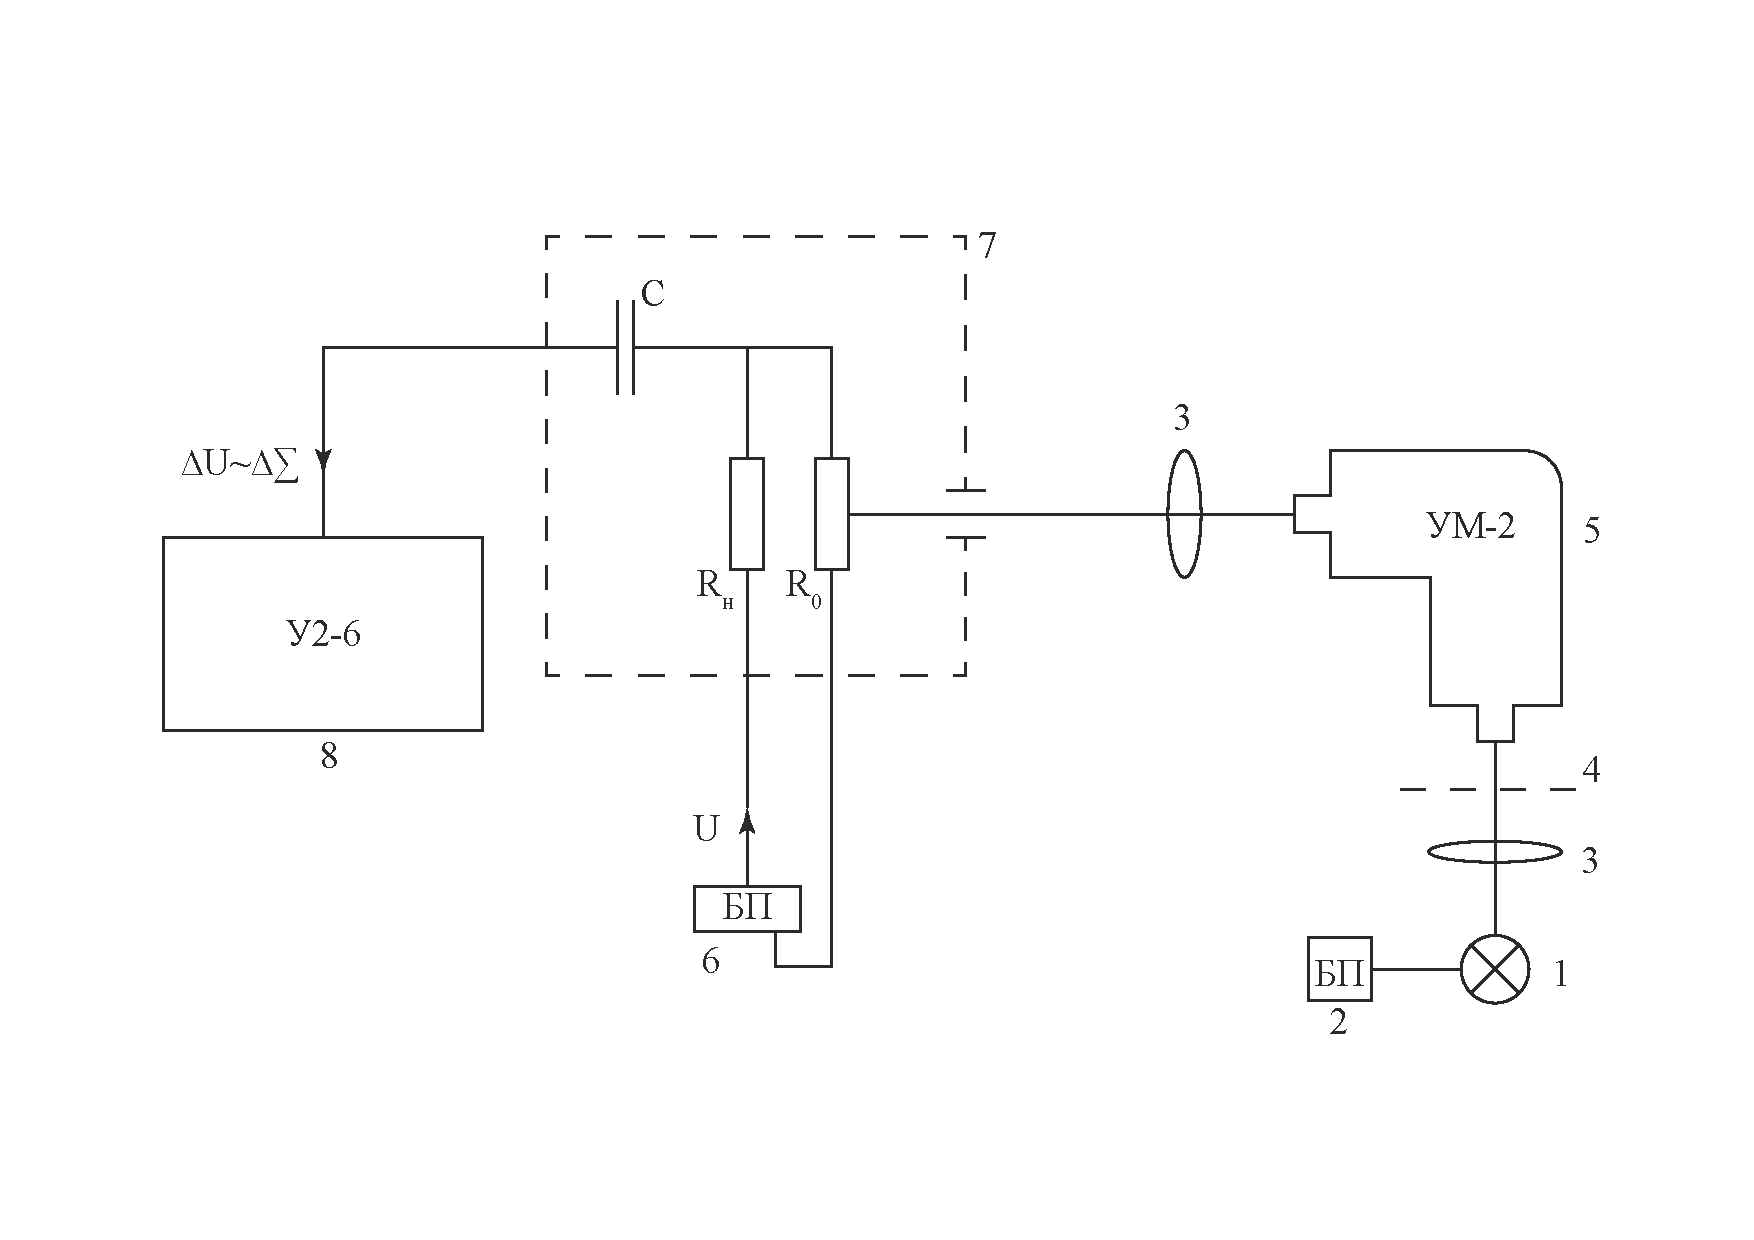
\includegraphics[width= 0.8\textwidth]{exp_scheme.pdf}
    \caption{Схема экспериментальной установки. 1 -- осветитель, 2 -- блок питания осветителя, 3 -- линзы, 4 -- механический модулятор излучения, 5 -- монохроматор, 6 -- блок питания образца, 7 -- схема включения образца, 8 -- усилитель}
\end{figure}
\section*{\textcolor{header}{Обработка экспериментальных данных}}

\subsection*{\textcolor{sub_header}{GaAs}}

\begin{figure}[htbp]
    \centering
    \includegraphics*[width = 0.9\textwidth]{raw.png}
    \caption{Экспериментальные данные для $GaAs$}
    \label{fig:exp_data}
\end{figure}

Экспериментальные данные изображены на рисунке $\ref{fig:exp_data}$. Для определение ширины запрещенной зоны построим зависимость логарифма обратного показателя пропускания.
\begin{figure}[htbp]
    \centering
    \includegraphics*[width = 0.9\textwidth]{main.png}
    \caption{зависимость логарифма обратного показателя пропускания от длины волны}
    \label{fig:GaAs}
\end{figure}

Как видно на рисунке \ref{fig:GaAs}, ширина запрещенной зоны $GaAs$ оказалась равной $1416 \text{ мэВ}$.


\subsection*{\textcolor{sub_header}{Ge}}

Аналогичный график построим для германия(смотрите рисунок \ref{fig:Ge}).

\begin{figure}[htbp]
    \centering
    \includegraphics*[width = 0.9\textwidth]{main_2.png}
    \caption{зависимость логарифма обратного показателя пропускания от длины волны}
    \label{fig:Ge}
\end{figure}

Как видно на рисунке \ref{fig:Ge}, ширина запрещенной зоны германия порядка $680 \text{ мэВ}$.


\section*{\textcolor{header}{Вывод}}
 Удалось определить ширину запрещенной зоны для GaAs и Ge. Экспериментально полученные значения, в пределах погрешности, сошлись с табличными. 





\end{document}
